\chapter{Related Work}

In this chapter, we will present several tools with similar focus as our proposed \emph{application generator}. That will help us to identify the key features that we will need to implement in order to achieve our goals. We aim to create a \emph{Linked Data-driven web application generator}. So we have to begin with defining what kind of tools would fall into the same category. Before we start: Let us not limit ourselves only to Linked Data based tools. Firstly, there is not that many similar Linked Data based tools available so there would not be much to analyze. Secondly, we can get interesting findings even from the other tools, as the inner data format is only one aspect of a generator (and for a non-developer, i. e., our potential user, it is definitely not the most important one). We will now move on to the individual features that a tool should have in order to be classified by us as a \emph{data-driven application generator}.

Firstly, such a tool should be a \emph{generator}. That means that whatever the generator produces, it should not disappear after the generator is closed and it should persist as an independent \emph{instance}. This requirement is rather vague as for example any text processor (e.g. Microsoft Word) would count as a generator in this sense. But it does rule out all kinds of \emph{data viewers}. Secondly, such a tool should generate \emph{applications}. An application, to be called an \emph{application}, should offer (at least potentially) some level of interactivity. For example text documents, images or static visualizations (like non-interactive graphs) are definitely not applications. Lastly, such a tool should be \emph{data-driven}. That means that in a typical scenario, one should start the process with a data set and use this data set to create a new application with the generator.  To give you an example of what we do not consider \emph{data-driven}, we could mention for example the WordPress.com \cite{wordpress} platform. This platform definitely is an \emph{application generator} according to our first two requirements (specifically, it is a \emph{website generator}, or perhaps a \emph{blog generator}). The key difference is that when you create a new application (a \emph{website} or a \emph{blog}), it is empty and then you start adding the data. The process is completely reversed.

We admit that all these definitions are rather vague and it can still be hard to determine whether a certain tool falls into the category of \emph{data-driven application generators} or not. We believe, however, that all these definitions together give the reader a decent idea of what we consider a \emph{data-driven application generator}.

To make the comparison more organized, we define a limited set of features that we will specifically focus on while examining the tools. An overview table showing the support of these features among all selected tools will be presented to the reader. Let us now give a short description of each chosen feature.

\begin{itemize}
\item \emph{Linked Data support}. Our \emph{application generator} is going to be Linked Data based and we consider this aspect one of its biggest assets. Therefore we are naturally interested in the \emph{Linked Data support} of other tools as well.
\item \emph{Extendability}. We want to know whether a particular tool can be programmatically extended to support new types of data and new corresponding types of applications. By a type of data we do not mean a different format (the data might or might not be represented in RDF, that is irrelevant at this moment) but a different \emph{semantic} meaning of the data. For example, if we decide that our generator should be able to recognize geospatial data and visualize them using an application in the form of a map, can we extend the generator in such a way? Also just because a particular tool is released under an Open-Source software license and therefore can be modified, we do not consider it \emph{extendable}. Such a tool has to be intentionally \emph{designed} as \emph{extendable} with clearly defined and documented plugin interface.
\item \emph{Data analysis}. We are interested in whether the generator analyses the input data in any way. Typically, such a generator can enable (or disable)  features of generated applications depending on the characteristics of the input data. Or it can give recommendations to the user about how the data can be visualized. We can say that such a generator \emph{understands} the data to a certain extent. By contrast, a generator that performs no analysis at all, leaves the whole generation process up to the user. Then there is the question whether the application is still \emph{generated} or rather just \emph{built} by the user.
\item \emph{Online sharing}. We want to know whether a generated application can be published online.
\item \emph{Non-developers friendly}. Here we are interested in whether the \emph{application generator} can be operated by a person with no technical knowledge. We are focused specifically on the actual application creation process. An expert might be needed to set up the generator, but this requirement would not break this condition.
\item \emph{Platform}. This feature specifies whether the generator exists in the form of an online \emph{platform} where each user has an account through which he can create, publish and manage his applications.
\item \emph{Configuration}. Here we want to know whether the generator will simply take the input data and generate and publish the application, or whether it will offer the user an extra \emph{configuration} step in between, in which the user will be able to affect the final shape of the application before publishing it. This configuration step should allow more than just changing the application name.
\end{itemize}

\def\checkmark{\tikz\fill[scale=0.4](0,.35) -- (.25,0) -- (1,.7) -- (.25,.15) -- cycle;}
\newcolumntype{C}{>{\centering}X} % Create new column type that centers the cell content
\begin{table}[ht]
  \caption{Features of related tools}
  \vspace{0.5cm}
  \label{tab:related-features}
\begin{tabularx}
  {\textwidth}{ |r|C|C|C|C|C|C|C| }
  \hline
      \begin{sideways}Tool\end{sideways} & 
      \begin{sideways}Linked Data support\end{sideways} &
      \begin{sideways}Extendability\end{sideways} &
      \begin{sideways}Data analysis\end{sideways} &
      \begin{sideways}Online sharing\end{sideways} &
      \begin{sideways}Non-developers friendly\end{sideways} &
      \begin{sideways}Platform\end{sideways} &
      \begin{sideways}Configuration\end{sideways} \tabularnewline \hline
  \hline
% 						&LD			&Extend		&Data analysis	&Sharing	&Non-devel	&Platform	&Config	
  Miga Data Viewer		&			& 			&\checkmark	 	&\checkmark &			&			&\checkmark ~ \tabularnewline \hline
  Citadel on the Move	& 			&\checkmark	&				&\checkmark	&\checkmark	&\checkmark	&\checkmark	~ \tabularnewline \hline
  Tableau       		& 			&			&				&\checkmark	&\checkmark	&\checkmark	&\checkmark	~ \tabularnewline \hline
  Avelca                & 			&			&				&\checkmark	&\checkmark	&\checkmark	&\checkmark	~ \tabularnewline \hline
  Exhibit             	&\checkmark	&\checkmark	&				&\checkmark	&			&			&\checkmark	~ \tabularnewline \hline
  Payola              	&\checkmark	&\checkmark	&				&\checkmark	&\checkmark	&\checkmark &\checkmark	~ \tabularnewline \hline
  LinkedPipes           &\checkmark	&\checkmark	&\checkmark		&\checkmark	&\checkmark	&\checkmark &			~ \tabularnewline \hline

\end{tabularx}
\end{table}

\section{Miga Data Viewer}

Miga Data Viewer is a tabular data based \emph{application generator}. It accepts only data in the CSV format but as this format is widely supported and there is lots of conversion tools available, any source of tabular data (Microsoft Excel file, RDBMS) can be used as an input. Despite the word \emph{viewer} in the name, this tool does meet our requirements to be called an \emph{application generator}. What it generates is an interactive interface that supports browsing, searching and filtering over the input data set. Once it is generated, it can be published online.

\begin{figure}
	\centering
	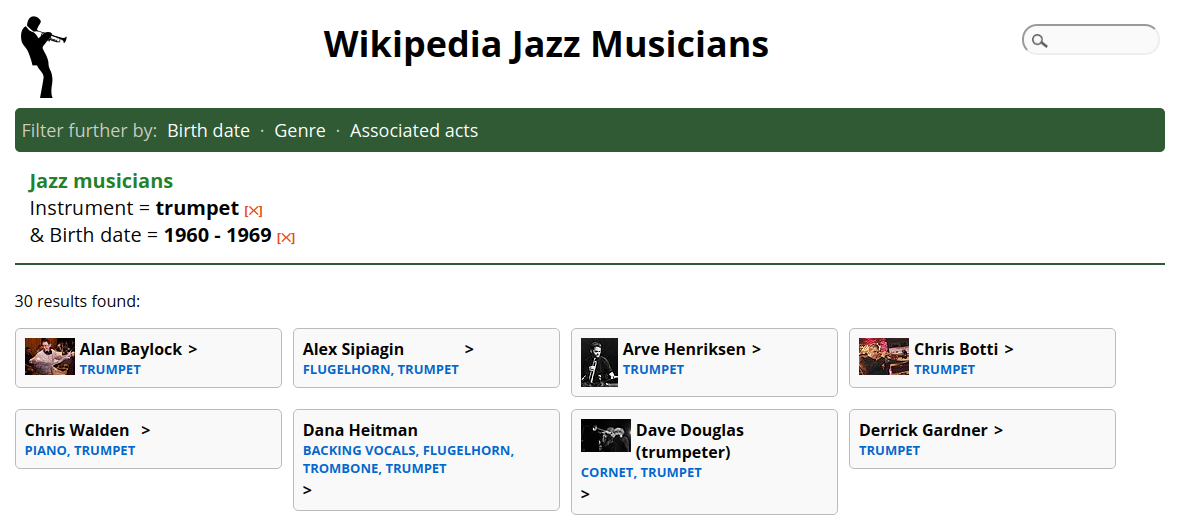
\includegraphics[width=140mm]{img/02_miga_data_viewer.png}
	\caption{Miga Data Viewer: A sample application generated from a set of Jazz Musicians.}
	\label{fig:miga-data-viewer}
\end{figure}

As we already mentioned in the introduction chapter, the big disadvantage of tabular data is that they carry very little semantic information. As without the semantic information, it would be almost impossible to generate anything else but a simple paginated table, the user is required to provide a \emph{schema definition} for each data table (for each single CSV file). That is done through configuration *.ini files using a custom \emph{Miga Data Schema} format. Here is an example of such a configuration:

\scriptsize
\begin{verbatim}
[Books]
Title = Name
Author = List (,) of Entity (Authors/Name)
Number of pages = Number
Genre = List (,) of Text
Wikipedia URL = URL

[Authors]
Name = Name
Birth date = Date
\end{verbatim}
\normalsize

Each section defines a schema for a CSV file with a name matching the section's name. Each column in the data file is assigned one of the data types provided by the \emph{Miga Data Schema}. Besides the very basic ones (\emph{Text} or \emph{Number} that correspond to data types known from programming languages) and slightly more complex ones (\emph{List} for collections, \emph{Entity} working as a \emph{foreign key} pointing to a different CSV file), there are a few special ones with added \emph{semantic meaning}. Let us name for example \emph{URL}, \emph{Image URL} or \emph{Coordinates} (GPS coordinates). Using these types the Miga Data Viewer is able to dynamically create richer interfaces (e.g. it can display entities with coordinates on a map).

It is clear that this format is the authors' attempt to solve what RDF would be perfect for. But unlike RDF, which is a universal, open and widely supported framework, this format will work with Miga Data Viewer only. We will see similar approaches in other generators as well.

Although creating an application does not require the user to know any programming language, the process does involve fairly low-level work with the *.ini schema files. Because of this we do not consider this tool \emph{non-developers friendly}.

When we ask whether this tool \emph{analyses} the data or \emph{understands} it in any way, it brings up an interesting point. In this case, it depends on whether we consider the schema to be part of the data set (as the schema is also a file, it can be distributed together with the data itself). If we do that, then we can say that the generator really \emph{understands} the data (to an extent). If it comes across GPS coordinates, thanks to the schema it will know that it is GPS coordinates, and as already explained, it will automatically add a map view to the generated application. On the other hand, if we consider the schema to be the application configuration, strictly separated from the data, then we cannot talk about any kind of \emph{understanding}. In this sense, the generator is told by the user to use a map view.

Because it is possible to put the schema and the data together, creating one package that can work as the generator input, we consider this tool to offer automatic (yet very simple) \emph{data analysis}.

\section{Citadel on the Move}

Citadel on the Move \cite{citadel_home} is a project \cite{citadel_paper} funded by European Commission. The presented goal is to simplify the process of generating Open Data based applications for both developers and non-developers, that provide useful city services. The idea behind this project was that an application providing a certain service (e.g. available park places) for one European city should be able to work just as well in another European city, only with a different data set. The applications generated by this tool are very simple map applications that work as interactive data viewers (similarly to Miga Data Viewer).
% * <tobiaspotocek@gmail.com> 2016-06-12T19:44:03.785Z:
%
% > Open Data
%
% How to reference this?
%
% ^.

\begin{figure}
	\centering
	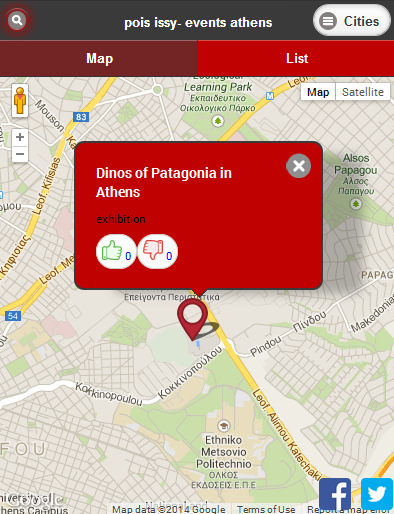
\includegraphics[width=80mm]{img/02_citadel_on_the_move_app.jpg}
	\caption{Citadel on the Move: A sample generated application. Source of picture \cite{citadel_agt_doc}}
	\label{fig:citadel-on-the-move}
\end{figure}

Citadel on the Move is not a monolithic application but a fairly large project consisting of several components.

\begin{itemize}
\item The project defines its own data set format called \emph{Citadel JSON}. As the name suggests, the data are serialized into JSON following a custom schema. Each data set contains a single list of entities where each entity has couple of mandatory fields (like a unique identificator, name or GPS coordinates necessary for the map visualization) plus an arbitrary number of optional attributes (which may vary depending on a data set and are not in any way defined by the schema). 
\item The project offers a \emph{Citadel table to JSON Converter tool} which allows the user to convert any tabular data (typically CSV or Microsoft Excel spreadsheet) into the internal \emph{Citadel JSON} format. Clearly, the original data set has to contain all required information. The tool just enables the user to create mappings between table columns of the original data set and the schema fields.
\item The core component is the \emph{Application Generator Tool} which allows non-developers to create their own applications in just couple of simple steps. They start by selecting a city (or cities) that they are interested in, they continue by selecting a data set (or data sets) available for the chosen city (or cities) and finally they just fill in basic app configuration (name, description, color scheme) to create the application. The generated application is an interactive interface that allows the user to browse, filter and see the data on a map (as said, similarly to Miga Data Viewer).
\item A part of the project is also a \emph{platform} in a form of an online portal available on the cited URL \cite{citadel_home}. It is wrapped around the  \emph{Application Generator Tool} and provides additional functionality like published applications catalog, user management, support etc.
\item The last component are customizable application \emph{templates}. If the application generated by the \emph{Application Generator Tool} is not sufficient, the user can instead manually instantiate a \emph{template} and configure it to use the given data set. This approach is completely separated from the \emph{Application Generator Tool}. It is not possible to select a template while generating an application. This has to be done manually and it requires certain programming skills. A distinct advantage is that using a template gives the user significantly bigger freedom of customization. E.g. it is possible to edit the application layout or upload a custom application logo. An example of such a special template is the \emph{Citadel Events Template} that extends the default application (which is used in the \emph{Application Generator Tool}) by a calendar which allows filtering over events contained in the data set (those are standard entities with couple extra attributes that are specified in the template documentation).
\end{itemize}

To sum it up: Citadel on the Move offers two different approaches. The first one utilizes the \emph{Application Generator Tool} which allows non-developers to generate simple applications in a very \emph{friendly} way. The other one utilizes the \emph{templates} which allow developers to create more customizable applications. There is no data \emph{analysis} involved. The user has to select a different template manually and he has to make sure that the given data set contains all necessary information that the template needs in order to work properly. The project offers several different documented templates and encourages the developers to create new ones which makes the project \emph{extendable}. As the \emph{templates} are just standalone web applications (not plugins), there is no interface that they would need to implement. However, they need to support the common \emph{Citadel JSON} format. Just like Miga Data Viewer, Citadel on the Move needs to address the problem that standalone tabular data contain almost no semantic information. To deal with that, it provides the \emph{JSON Converter tool} which allows the user to map the data set table columns onto the Citadel JSON scheme.

\section{Tableau Software}

Tableau Software \cite{tableau} is a company behind a family of professional commercial products focused on rich interactive data visualizations. The core product is Tableau Desktop. It can be used together with Tableau Server, which adds sharing, collaboration and other features useful for organizations, or with Tableau Online which is Tableau Server hosted directly by Tableau Software (i.e. cloud solution). There is also Tableau Public which offers a light-weight free version of Tableau Desktop and focuses on creating rich online public visualizations.

\begin{figure}
	\centering
	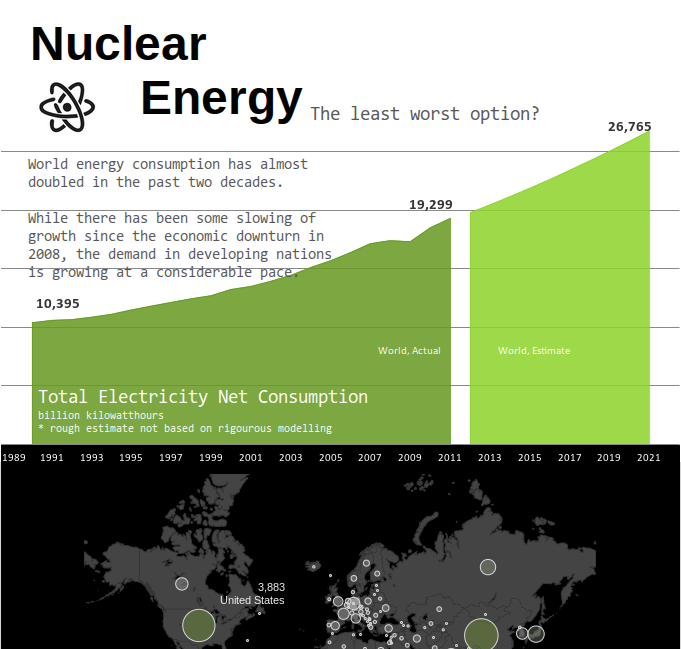
\includegraphics[width=110mm]{img/02_tableau_sample.png}
	\caption{Global Nuclear Energy Use \cite{citadel_agt_doc}. Sample rich interactive visualization created with Tableau Public}
	\label{fig:tableau-global-nuclear-enery-use}
\end{figure}

At first glance, Tableau Desktop has more in common with Microsoft Excel than with the \emph{application generators} we are describing in this chapter. A task typical for Tableau Desktop is to create a graph from a given data table. But this tool goes way beyond that. Firstly, it does not have to be just graphs. The user can choose from a very long list of rich and attractive visualizations. Secondly, the visualizations can very often be interactive, allowing easy data exploration. And lastly, multiple visualizations can exist within a single document. They can be arbitrarily combined and put into a layout chosen by the user.

A typical output of Tableau Desktop is an interactive \emph{dashboard} containing multiple visualizations. The \emph{dashboard} can be extended with filtering tools that control the underlying data set. As the end user changes the filters, the visualizations on the \emph{dashboard} change on-the-fly. The Tableau Desktop is not promoted as \emph{application generator} but given the nature of produced \emph{dashboards} it can be very well considered as one. With little effort (and with no developer knowledge) it can achieve very similar results as the previously described generators, Miga Data Viewer and Citadel on the Move.

It works only with tabular data but unlike the previous tools, it supports by default many various source types. Besides the classical ones like Microsoft Excel spreadsheets or CSV, it allows the user to connect to live databases (the published dashboards can work as live views on the database content). Tableau Desktop contains many \emph{analytical} (and statistical) tools but not in the sense that they would dynamically help the user with creating the visualizations. The process is very \emph{user-friendly} (overall drag and drop approach) but it is completely controlled by the user. The application is not really \emph{generated}, the user \emph{builds} it.

We can assume that the inner software architecture does support extending, but as it is a commercial closed source product, there is no natural way in which a user could extend the generator with features he would desire. He can only rely on the authors.

\section{Avelca}

Avelca \cite{avelca} is another commercial tool for building custom business applications. Among the tools that we are describing in this chapter, this one is probably the furthers from our original definition of a \emph{data driven application generator}. It is focused on companies and organizations allowing them to build interactive applications around their agendas. An example of an application created with this tool could be a movie rental database, keeping track of owned movies, registered customers and current rentals. Thanks to Avelca, even a user with zero developer knowledge can create such an application.

\begin{figure}
	\centering
	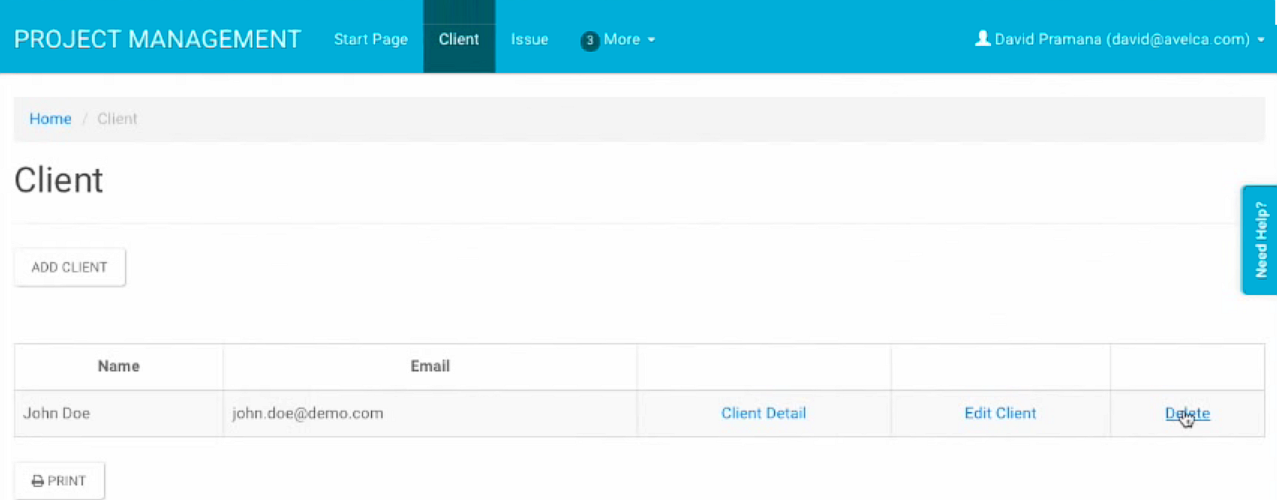
\includegraphics[width=110mm]{img/02_avelca.png}
	\caption{Sample application generated with Avelca. Source: YouTube demo video \cite{avelca_youtube}}
	\label{fig:avelca-example}
\end{figure}

In its essence, Avelca \emph{application generator} is just a \emph{user-friendly} interface over a common relational database. The user starts with creating the database schema, i.e., creating tables and defining relationships between them. Obviously, the interface is more verbose and uses vocabulary that is friendlier (it avoids the standard technical terms) in order not to scare off the non-developer user. The generator then uses the schema definition to create the actual application. Another way is to start with an existing data source (once again, only tabular data are supported, typically Microsoft Excel spreadsheet) and use it as a base for the generated application. This feature puts this tool among our \emph{application generators} but you should note that this time, starting with a data set is just an option, the user can actually begin with an empty application and use it to create the data.

Avelca is a proprietary Application Platform as a Service. That means that on one hand, \emph{online sharing} is supported by default, on the other, it is not possible to \emph{extend} the generator in the sense that we described at the beginning of this chapter. There is also no actual \emph{data analysis} going on. The application is completely built by the user. The only exception might be the situation when the tabular data are being imported and Avelca has to \emph{guess} the table schema. That process is, however, very straightforward and we can hardly speak about some kind of \emph{understanding} of the data.

In a way, Avelca is very similar to the Miga Data Viewer. Both tools work with tabular data that are augmented with a schema definition effectively turning it into some kind of relational database. The application is then generated from both the data and the schema. Clearly, Avelca is a way more advanced tool (Miga Data Viewer is just an interactive viewer) but the particular difference we are interested in at this moment, is that to achieve the same (i.e., defining the schema), they use two different approaches. Miga Data Viewer requires the user to create the schema using *.ini files, whereas Avelca offers a rich, user-friendly, drag and drop-based interface (interestingly enough, the underlying technology in Avelca uses YAML-based DSL to represent the schema).

This creates a little paradox. Miga Data Viewer \emph{feels} a bit more like an \emph{application generator} than Avelca. You start with a data set, augment it with a schema defined in a small and simple file and that is it. Miga Data Viewer generates the application from these two pieces of information. Moreover as already explained, if we consider the schema definition to be a \emph{part} of the data itself, then we can say that Miga Data Viewer actually \emph{understands} the data \emph{semantics} and uses this ability to create better and richer applications. This can be hardly claimed about Avelca. We can say that the Miga Data Viewer schema definition is part of the data only because it is an actual file that can be distributed with the data. In the case of Avelca, the schema definition is stored somewhere on the Avelca servers and the user can access it only through the user interface. It is definitely not part of the data. On top of that, the whole process of creating an application is very different and it feels more like \emph{building} than \emph{generating}. But besides all of this, the fact remains that Avelca can be used to get very similar results to what you can do with Miga Data Viewer. Avelca is like an upgraded and more advanced Miga Data Viewer with a slightly different overall approach.

We understand that his is very subjective. We are mentioning this paradox here only to show that it is hard to define and agree on what a \emph{application generator} is and that there are many different tools that might share some of the features we are interested in, but not all of them.

\section{Exhibit}

Exhibit 3.0 \cite{exhibit} is a publishing framework for large-scale data-rich interactive Web pages. It offers yet another approach compared to what we have seen so far. To see how it works, we will have a look at a sample application "Billionaires in History" \cite{exhibit_example}. The data are in Exhibit internal JSON-based format (which we will mention later) but in their nature it is just a simple 2D table containing a list of billionaires with several named properties (name, age, wealth, origin etc). The \emph{applications} produced by Exhibit are called \emph{exhibits} and they are directly embedded into HTML pages. So when creating an \emph{exhibit} like the mentioned "Billionaires in History" application, we would start with an empty HTML page. In the first step, it is necessary to link \emph{Exhibit JavaScript API} and the actual data set into the page. For this particular application, we also need to link an Exhibit plugin with the map view. Once this is done, we can start inserting Exhibit widgets and components into the HTML page using special syntax.

\begin{figure}
\centering

  \begin{verbatim}
  <div ex:role="view"
    ex:viewClass="Map"
    ex:label="Where They Are From"
    ex:latlng=".latLng"
    ex:sizeKey=".wealth"
    ex:sizeCoder="wealth-coder"
    ex:bubbleWidth="200"
    ex:bubbleHeight="200"
    ex:bubbleTip="top"
    ex:mapHeight="500"
    ex:sizeLegendLabel="Wealth in Billion USD"
    >
      <div class="map-lens" ex:role="lens" style="display: none;">
        <div>
          <b ex:content=".label"></b>
          <span ex:if-exists=".origin">
          	from <span ex:content=".origin"></span>
          </span>
        </div>
        <div><span ex:content=".wealth"></span> billions USD</div>
        <div>Company: <span ex:content=".company"></span></div>
      </div>
  </div>
  \end{verbatim}  
  \caption{Code snippet from the "Billionaires in History" application \cite{exhibit_example} showing how the map is instantiated.}
  \label{fig:exhibit-map-code-snippet}
\end{figure}

As you can see in Figure \ref{fig:exhibit-map-code-snippet}, the special syntax consists of standard HTML tags extended with custom attributes prefixed with \texttt{ex:}. We insert the map into our application by creating a new wrapping \texttt{div} tag and giving it the attributes \texttt{ex:role="view"} and \texttt{ex:viewClass="Map"}. 

The map should display a \emph{bubble} for each billionaire. The size of the \emph{bubble} corresponds to the billionaire's wealth and the position of the \emph{bubble} corresponds to the coordinates of his origin. This mapping is specified using the \texttt{ex:sizeKey} and \texttt{ex:latlng} attributes, i.e., the \texttt{ex:sizeKey} attribute says that the \emph{bubble} size should be defined by the \texttt{wealth} property, and the \texttt{ex:latlng} attribute says that the \emph{bubble} position should be defined by the \texttt{latLng} property. The child \texttt{div} with the \texttt{ex:role} attribute set to \texttt{lens} defines the looks and the contents of a \emph{bubble tooltip}  which is displayed upon a click on the \emph{bubble}. Notice how the data properties are linked to the code using the \texttt{ex:content} attribute. 

\begin{figure}
	\centering
	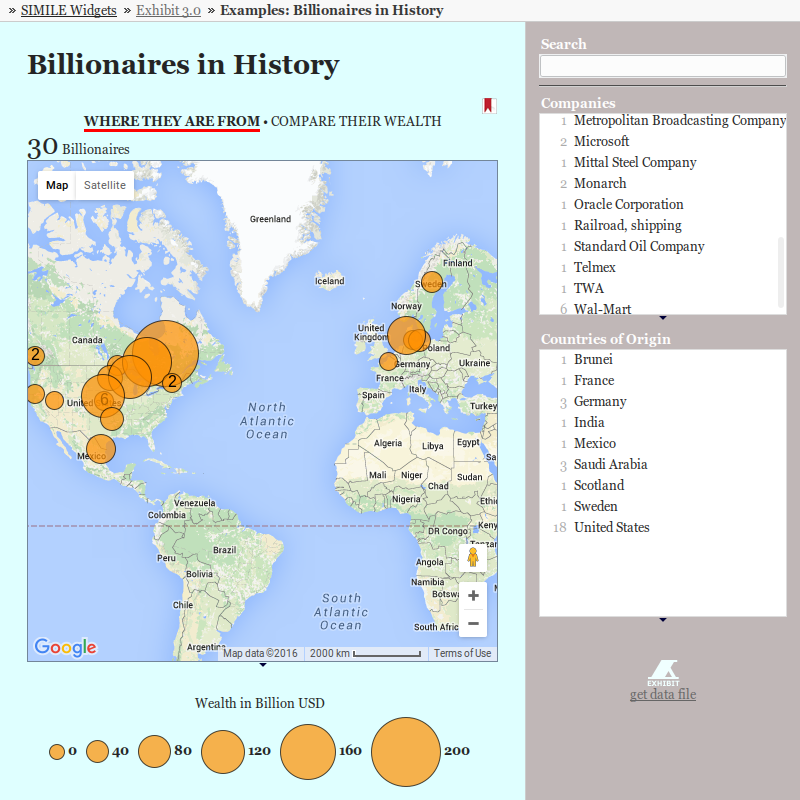
\includegraphics[width=110mm]{img/02_exhibit.png}
	\caption{"Billionaires in History" application \cite{exhibit_example} created with Exhibit.} 
	\label{fig:exhibit-map-example}
\end{figure}

Exhibit provides a large number of available components and widgets which can be used to create complex and interactive applications. As the components can be combined with standard HTML and CSS markup, the user has almost unlimited possibilities in how the final application should look like. The obvious disadvantage is that the user has to have at least some basic knowledge of HTML in order to be able to create an application with Exhibit. That means that Exhibit is not really \emph{non-developers friendly} but on the other hand, no real programming skills are needed and even with a shallow knowledge of HTML, one can achieve very good results.

In the previous cases of \emph{application generators}, we were examining how they deal with missing \emph{semantic} information. For example, Miga Data Viewer requires a schema definition which allows the user to specify the extra \emph{semantic} information. If a data property is marked as GPS coordinates, Miga Data Viewer displays the appropriate entity on a map. Exhibit has an exactly opposite approach. The user assigns the meaning to individual properties by using them \emph{properly} in component configuration. If you have a look at the map example, what happens there is that we tell the map widget that the \texttt{latLng} property contains GPS coordinates. Nevertheless, besides this approach, Exhibit does allow us to create a schema for our data as well. Typically, the schema can define how entities of different types are related to each other within a single data set.

Internally, Exhibit uses its own JSON-based data format which makes it possible for the data to live together with the schema within a single file. We have seen a similar approach with a custom format in Citadel on the Move. Just like Citadel on the Move, Exhibit also offers tools allowing arbitrary data sets to be converted into the internal format. This time, however, the internal format is way more powerful, so the original data sources are not limited to just tabular data. For example, \emph{Linked Data} are also supported by Exhibit.

As Exhibit consists of individual components and widgets, it can be naturally extended by adding new components and new widgets capable of displaying new types of data. For those who decide to extend Exhibit, there is developer documentation available \cite{exhibit_documentation}.

\section{Payola}

Payola \cite{payola} is an online all-in-one platform for reading, sharing, analyzing and visualizing LinkedData. It is a technological predecessor of another tool, LinkedPipes, on top of which our \emph{application generator} is going to be built. At first glance Payola might not look like an \emph{application generator} the way we defined it and its purpose is really slightly different, but it can be used as one.

\begin{figure}
	\centering
	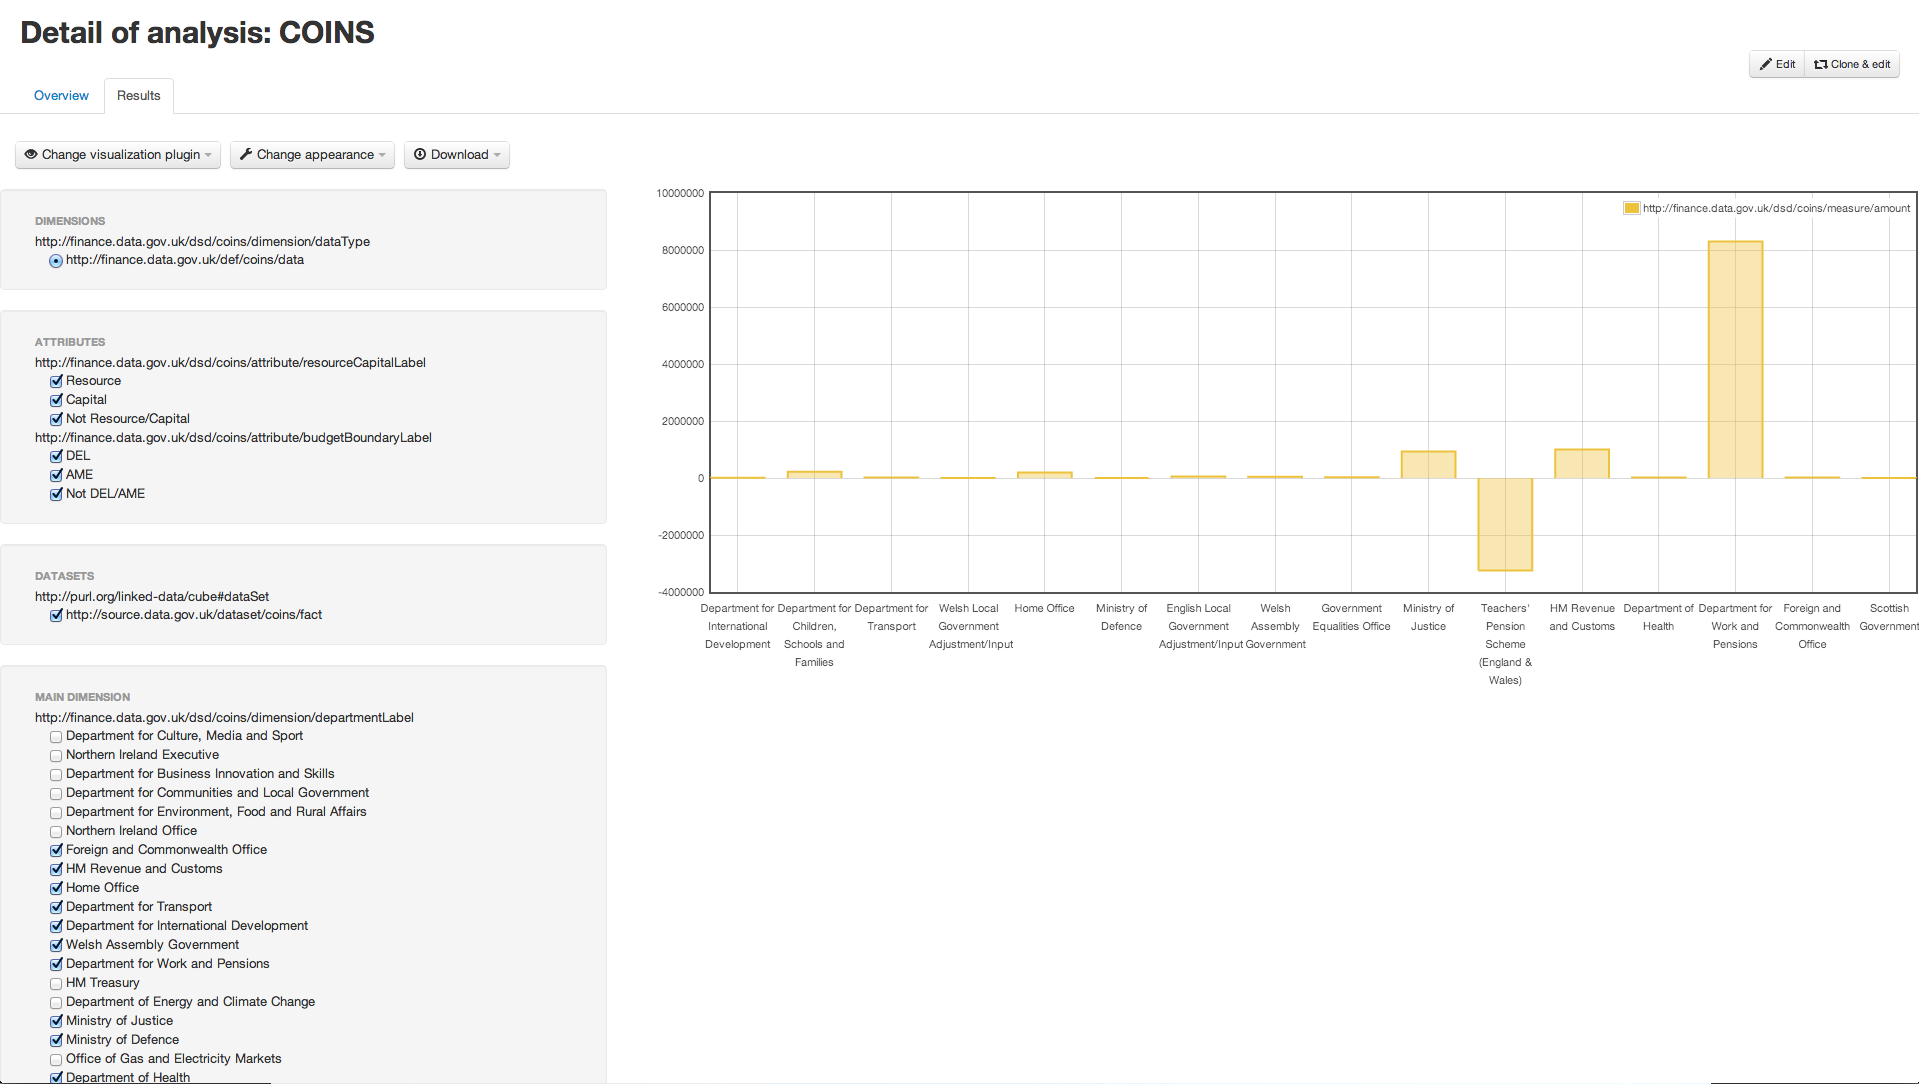
\includegraphics[width=150mm]{img/02_payola.png}
	\caption{Sample visualization created with Payola. Source: Payola User Guide \cite{payola_user_guide}} 
	\label{fig:payola-example}
\end{figure}

Using Payola, the user can build his own Linked Data \emph{analyses}. An \emph{analysis} is a hierarchical tree-like structure of plugins with a single output and multiple data inputs bound to different RDF data sources. Each plugin has an input (or multiple inputs) and it represents an operation that is applied on the input data. The idea is that the user can use the plugins to filter, search and combine the data from all the sources. By building the hierarchy of plugins, the user creates a \emph{pipeline} which can be understood as an algorithm specifying how the input data should be processed. The result of such an \emph{analysis} are also valid RDF data.

The result can be visualized using several available \emph{visualization plugins}. Some of them are interactive allowing the user to play with the \emph{analysis pipeline} output. When we talk about Payola as an \emph{application generator}, this is what we have in mind. Payola can be used to generate interactive visualizations from RDF data. The generated visualizations can be shared online using the platform features.

Unlike the previously described tools, Payola puts a lot of emphasis on the work with the data itself. All the other tools simply took the given input data source and tried to generate an application form it. Payola with its \emph{analyses}, on the other hand, leverages the distributed nature of Linked Data and offers the user a way to build his own data sources before visualizing it (that is the \emph{analysis pipeline} output). There is an interesting paradox that even though Payola allows the user to build his own \emph{analyses}, it does not perform any \emph{analysis} on its own, i.e., it does not try to \emph{understand} the data. It is completely up to the user to explore the data, build the \emph{analysis pipeline} and apply an appropriate visualization plugin.
% * <tobiaspotocek@gmail.com> 2016-06-14T20:23:26.071Z:
%
% > does not perform any \emph{analysis} on its own
%
% I hope this is a correct statement.
%
% ^.

The final visualization is what we consider the \emph{generated application}. As such, it is not configurable in similar manner as in the previously described \emph{application generators}, i.e., it is not possible to take the \emph{analysis pipeline} output, select a visualization plugin and start building an application from it. But as the analytical process is completely controlled by the user, he can add various plugins to the \emph{analysis pipeline}, in order to alter the data output which will eventually change the visualization itself. From this perspective, the visualization can be \emph{configured} to a certain extent .

The process of creating an \emph{analysis pipeline} involves instantiating individual plugins, configuring them and binding them together. It is all done through a clickable user interface. Some basic knowledge of how Linked Data work is required, nevertheless, we would still classify the process as \emph{non-developer friendly}. On the other hand, in order to be able to perform more complex operations with the data, the user needs to be able to construct custom \texttt{SPARQL} queries.

Payola is easily extendable by new analytical and visualization plugins. The analytical plugins can be even added directly through the web interface.

\section{LinkedPipes Visualization}

LinkedPipes Visualization is a successor of Payola. It is also a platform for reading, sharing, analyzing and visualizing Linked Data. As our \emph{application generator} is going to be built on top of LinkedPipes Visualization, we will dedicate one whole chapter to this tool and here we will give just a short description.

In Payola, the user has to manually build the \emph{analytical pipeline} by combining available plugins and applying them on input data sources. In LinkedPipes Visualization, the user just selects the RDF data sources and the tool will automatically discover all possible combinations of available plugins, making up \emph{pipelines} that lead to meaningful visualizations. For example, if the data set contains geospatial information, LinkedPipes Visualization will automatically offer the user a map visualization of the data. Or if the data set contains geospatial information in a format that the map visualization plugin does not understand, but there is a plugin available that can transform the data into the required format, LinkedPipes Visualization will automatically insert that plugin into the \emph{pipeline} and that \emph{pipeline} will be offered to the user.

Compared to Payola, this approach is way more \emph{non-developers} friendly and also faster as it does not involve the slow manual process of creating the \emph{analysis pipeline}. On the other hand,  the automatically generated pipeline cannot be altered or configured in any way which means that also the visualization cannot be configured. The user has to rely on the plugins that are currently available. The only way around this is to create and add a new plugin, but that is significantly more complicated and requires developer knowledge.